\documentclass[border=3pt]{standalone}
\usepackage{tikz}
\usetikzlibrary{arrows.meta,calc}
\tikzset{pin/.style={-{Stealth[length=5pt]}}}
\begin{document}
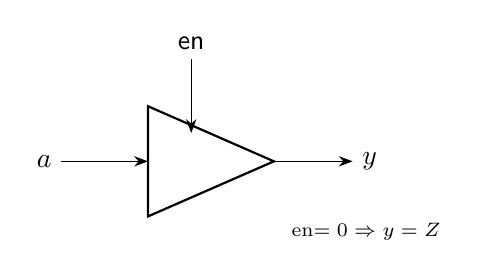
\begin{tikzpicture}[font=\sffamily]
  % buffer triangle
  \draw[thick] (0,0.7) -- (0,-0.7) -- (1.6,0) -- cycle;
  \draw[pin] (-1.1,0) node[left]{$a$} -- (0,0);
  \draw[pin] (1.6,0) -- ++(1.0,0) node[right]{$y$};
  % enable from top to apex of triangle
  \draw[pin] (0.55,1.3) node[above]{en} -- (0.55,0.36);
  \node[font=\scriptsize, right] at (1.7,-0.9) {en$=0\Rightarrow y=Z$};
\end{tikzpicture}
\end{document}
